\documentclass{article}
\usepackage{graphicx}
\usepackage[margin=1.5cm]{geometry}
\usepackage{amsmath}

\begin{document}
\twocolumn

\title{Wednesday Warm Up: Resistors in Series/Parallel, Kirchhoff's Rules}
\author{Prof. Jordan C. Hanson}

\maketitle

\section{Memory Bank}

\begin{itemize}
\item $\Delta V = I R$ ... Ohm's Law.
\item $R_{\rm tot} = R_1 + R_2 + ...$ ... Resistors \textit{in series}
\item $R_{\rm tot}^{-1} = R_1^{-1} + R_2^{-1} + ...$ ... Resistors \textit{in parallel}
\item Kirchhoff's Rule \#1: Total current into a junction equals total current out of a junction.
\item Kirchhoff's Rule \#2: The total change in voltage around a loop is zero.
\end{itemize}

\section{Resistors in Series/Parallel, Kirchhoff's Rules}

\begin{enumerate}
\item Consider Fig. \ref{fig:1}.  (a) If $V_0 = 12$ V, and the resistance of bulb B is $R_{\rm B} = 5$ $\Omega$, what current flows if the switch in the middle is open? (b) If $R_{\rm A} = R_{\rm B}$, what is the total resistance if the switch is closed? (c) What current flows if the switch is closed? \\ \vspace{5cm}
\item What is the power consumption if the switch is (a) open, (b) closed? \\ \vspace{5cm}
\item Repeat the previous two exercises, but let $V_0 = 5$ V, $R_{\rm A} = 4$ $\Omega$, and $R_{\rm B} = 8$ $\Omega$. \\ \vspace{5cm}
\item (a) What would the power consumption be if a third bulb was added in parallel with the first two, and each had a resistance of 5 $\Omega$? (b) Argue that the result makes sense in light of the conservation of energy. (c) What current would flow if the three bulbs were instead connected in series? (d) What would be the power consumption in that case?
\end{enumerate}

\begin{figure}
\centering
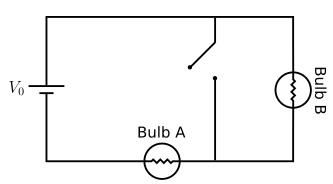
\includegraphics[width=0.45\textwidth]{figures/bulbs.png}
\caption{\label{fig:1} Two light bulbs connected to an EMF $V_0$.}
\end{figure}

\end{document}
